%%%%%%%%%%%%%%%%%%%%%%%%%%%%%%%%%%%%%%%%%%%%%%%%%%%%%%%%%%%%%%%%%%%%%%%%%%%%%%%
% PLANTILLA DE INFORME TÉCNICO - WASAFF CONSULTING
% VERSIÓN 1.0: DESAFÍO TÉCNICO-ACADÉMICO DEL MANIFOLD
%%%%%%%%%%%%%%%%%%%%%%%%%%%%%%%%%%%%%%%%%%%%%%%%%%%%%%%%%%%%%%%%%%%%%%%%%%%%%%%

\documentclass[11pt, a4paper,oneside]{article}

%=============== PREÁMBULO: CONFIGURACIÓN DEL DOCUMENTO =======================

\usepackage[utf8]{inputenc}
\usepackage[spanish, es-tabla]{babel}
\usepackage{graphicx}
\usepackage{geometry}
\usepackage{xcolor}
\usepackage{fancyhdr}
\usepackage{titlesec}
\usepackage{booktabs}
\usepackage{hyperref}
\usepackage[most]{tcolorbox}
\usepackage{parskip}
\usepackage{microtype}
\usepackage{amsmath} % Para un mejor formateo de ecuaciones
\usepackage{siunitx}

% --- Geometría y Colores ---
\geometry{a4paper, left=2.5cm, right=2.5cm, top=2.5cm, bottom=2.5cm, headheight=38pt}
\definecolor{WasaffNavy}{HTML}{001F3F}
\definecolor{WasaffCopper}{HTML}{B87333}
\definecolor{LightGray}{HTML}{F5F5F5}

% --- Fuentes y Títulos ---
\usepackage{lmodern} 
\usepackage{tgheros} 
\renewcommand*\familydefault{\sfdefault}
\titleformat{\section}
  {\normalfont\Large\bfseries\color{WasaffNavy}}
  {\thesection.}{1em}{}
\titleformat{\subsection}
  {\normalfont\large\bfseries\color{WasaffCopper}}
  {\thesubsection.}{1em}{}
\renewcommand*\familydefault{\rmdefault} 

% --- Encabezado y Pie de Página ---
\pagestyle{fancy}
\fancyhf{}
\fancyhead[L]{
\includegraphics[height=1cm]{wasaff_logo.png}}
\fancyhead[R]{\color{gray}\fontsize{9}{11}\selectfont \begin{tabular}{r} DESAFÍO TÉCNICO \\ \textit{Análisis de Flujo en Manifold Industrial} \end{tabular}}
\fancyfoot[C]{\color{gray}\thepage}
\renewcommand{\headrulewidth}{0.4pt}

% --- Configuración de Hyperref ---
\hypersetup{
    colorlinks=true, linkcolor=WasaffNavy, urlcolor=WasaffCopper,
    pdftitle={Análisis Comparativo de Distribución de Flujo en un Manifold Industrial},
    pdfauthor={Felipe Wasaff - Wasaff Consulting}
}

% --- Cajas de texto personalizadas ---
\tcbuselibrary{skins}
\newtcolorbox{problembox}{
    enhanced, colback=LightGray, colframe=WasaffNavy, fonttitle=\bfseries, arc=1mm, boxrule=0.5pt,
    title={Enunciado del Problema Académico}, top=3mm, bottom=3mm
}

%=============== DOCUMENTO PRINCIPAL =========================================
\begin{document}
\sffamily

% --- BLOQUE DEL TÍTULO ---
\
\vspace{1cm}
{\color{WasaffCopper} \large \textbf{INFORME TÉCNICO}}\\
\
{\color{WasaffNavy} \huge \textbf{Análisis Comparativo de Flujo en un Manifold Industrial}}\\
\
\vspace{1cm}
\
\rmfamily
\begin{tabular}{@{}p{14cm}}
    \textbf{Autor:} Felipe Wasaff \\
    \textit{Fundador, Wasaff Consulting} \\
    \href{mailto:felipe@wasaffconsulting.com}{felipe@wasaffconsulting.com} \\
\end{tabular}
\vspace{1cm}

\begin{problembox}
\textbf{Resumen:} Se desea caracterizar el comportamiento de un flujo incompresible y newtoniano a través de un manifold industrial. Se realizará un análisis comparativo de la caída de presión total ($\Delta P$) y la distribución de caudal ($Q_i$) en las cinco salidas utilizando tres metodologías de rigor creciente: cálculo analítico-empírico, Simulación por Elementos Finitos (FEM) y Simulación por Volúmenes Finitos (FVM).

\subsection*{1. Datos Geométricos}
\begin{itemize}
    \item \textbf{Material de la Tubería:} Acero Comercial (Rugosidad absoluta, $\epsilon = 0.045$ mm).
    \item \textbf{Tubería de Entrada (Header):} Diámetro Interno $D = 100 \text{ mm}$.
    \item \textbf{Tuberías de Salida (5):} Diámetro Interno $d = 50 \text{ mm}$.
\end{itemize}

\subsection*{2. Propiedades del Fluido (Agua a 20°C)}
\begin{itemize}
    \item \textbf{Densidad ($\rho$):} $998.2 \text{ kg/m}^3$.
    \item \textbf{Viscosidad Dinámica ($\mu$):} $1.002 \times 10^{-3} \text{ Pa}\cdot\text{s}$.
\end{itemize}

\subsection*{3. Condiciones de Contorno (Boundary Conditions)}
\begin{itemize}
    \item \textbf{Entrada (Inlet):} Perfil de velocidad uniforme y normal, $V_{in} = 1.0 \text{ m/s}$.
    \item \textbf{Salidas (Outlets):} Presión manométrica fija, $P_{out} = 0 \text{ Pa}$.
    \item \textbf{Paredes (Walls):} Condición de no deslizamiento (velocidad = 0 m/s).
\end{itemize}
\end{problembox}

%%%%%%%%%%%%%%%%%%%%%%%%%%%%%%%%%%%%%%%%%%%%%%%%%%%%%%%%%%%%%%%%%%%%
% REEMPLAZA LA SECCIÓN 1 COMPLETA CON ESTE CÓDIGO
%%%%%%%%%%%%%%%%%%%%%%%%%%%%%%%%%%%%%%%%%%%%%%%%%%%%%%%%%%%%%%%%%%%%

\section{Metodología 1: Solución por Cálculos Manuales}

\subsection{Planteamiento y Metodología}
El enfoque analítico-empírico busca aproximar el comportamiento del sistema utilizando ecuaciones fundamentales y datos experimentales consolidados (factores de fricción y coeficientes de pérdida). El análisis se basa en la aplicación simultánea de los principios de conservación de masa y de energía.

\begin{figure}[h!]
    \centering
    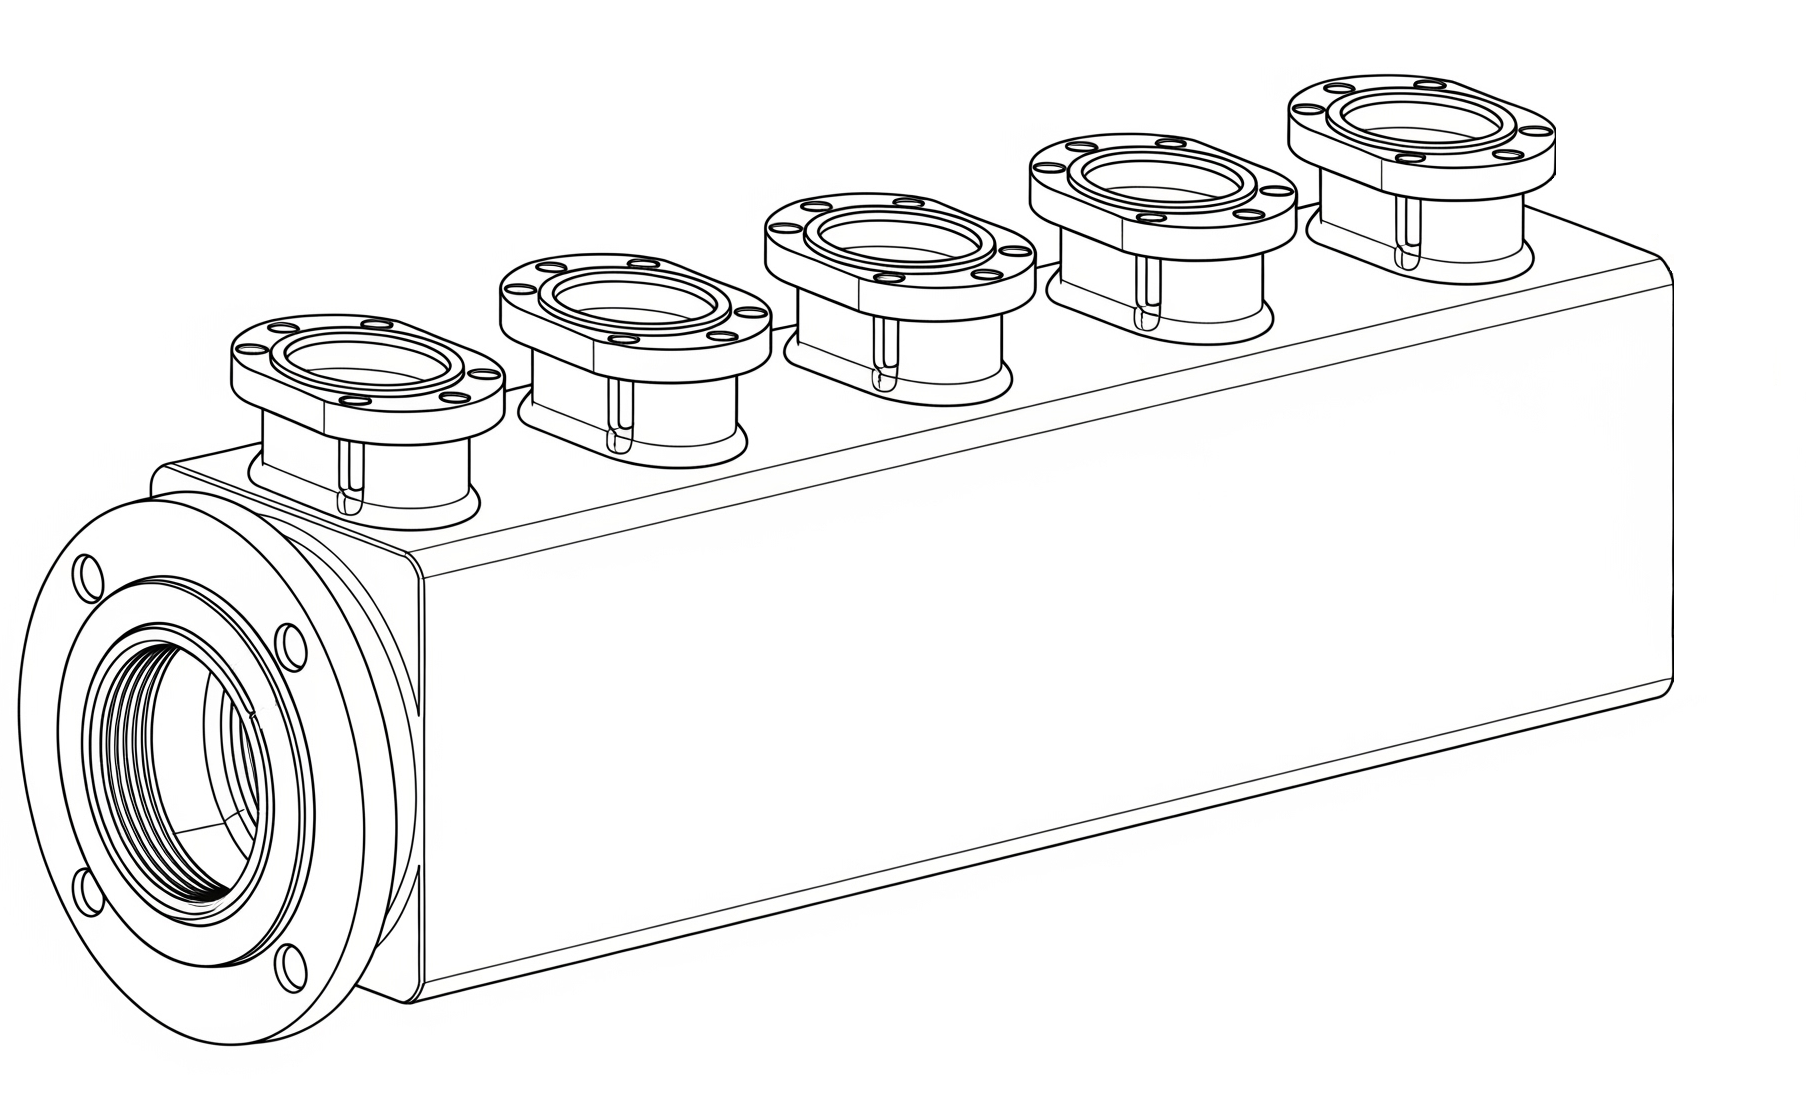
\includegraphics[width=0.8\textwidth]{manifold_render.png} 
    \caption{Esquema conceptual del manifold rectangular bajo análisis. Se ilustra la entrada principal y las cinco salidas superiores equidistantes, coincidiendo con la geometría del enunciado.}
    \label{fig:esquema_manifold}
\end{figure}

\subsubsection{Caracterización del Flujo}
El primer paso indispensable es determinar el régimen de flujo en la tubería de entrada para seleccionar las correlaciones adecuadas. Esto se logra calculando el número de Reynolds (Re):
\begin{equation}
    \text{Re} = \frac{\rho V D}{\mu}
\end{equation}
Donde los parámetros son tomados directamente del \textit{Enunciado del Problema Académico}. Sustituyendo los valores, obtenemos un número de Reynolds de aproximadamente \textbf{99,620}. Dado que $\text{Re} > 4000$, el flujo se encuentra en un régimen \textbf{turbulento}, como es esperado en la mayoría de las aplicaciones industriales.

\subsubsection{Ecuaciones Fundamentales}
El sistema se resuelve aplicando dos principios clave:

\textbf{1. Conservación de Masa:} El caudal total que entra al manifold ($Q_{in}$) debe ser igual a la suma de los caudales que salen por las cinco tuberías ($Q_i$).
\begin{equation}
    Q_{in} = \sum_{i=1}^{5} Q_{i} \quad \text{o} \quad A_{in}V_{in} = \sum_{i=1}^{5} A_{i}V_{i}
\end{equation}

\textbf{2. Conservación de Energía:} Se utiliza la Ecuación de Bernoulli extendida entre el punto de entrada (in) y cada una de las salidas (i):
\begin{equation}
    \frac{P_{in}}{\rho g} + \frac{V_{in}^2}{2g} + z_{in} = \frac{P_{i}}{\rho g} + \frac{V_{i}^2}{2g} + z_{i} + h_{L,total,i}
\end{equation}
Donde $h_{L,total,i}$ representa la totalidad de las pérdidas de carga que experimenta el fluido en su camino desde la entrada hasta la salida $i$.

\subsubsection{Cálculo de las Pérdidas de Carga ($h_{L}$)}
Las pérdidas se dividen en mayores (fricción) y menores (accesorios).
\begin{itemize}
    \item \textbf{Pérdidas Mayores (Fricción):} Se calculan con la ecuación de Darcy-Weisbach, donde el factor de fricción ($f$) se obtiene de la ecuación implícita de Colebrook-White.
    \item \textbf{Pérdidas Menores (Accesorios):} Se estiman con el Método de Coeficiente de Pérdida (K). \textit{Este es el punto de mayor simplificación.} El manifold se modela como una serie de uniones en "T". Críticamente, este método asume que cada unión es un evento independiente, \textbf{ignorando los efectos de interacción} entre las salidas consecutivas.
\end{itemize}

\subsubsection{Planteamiento del Sistema y Solución}
Se plantea un sistema de 6 ecuaciones con 6 incógnitas (5 caudales de salida y la presión de entrada). Dado el carácter no lineal e implícito de las ecuaciones, se resuelve de forma iterativa mediante un script computacional (Python), que ajusta la distribución de caudal hasta que la presión de entrada calculada para cada una de las cinco rutas converge a un valor único.

\subsection{Resultados y Discusión}
Tras ejecutar el proceso iterativo, el modelo numérico convergió en 52 iteraciones, revelando los resultados cuantitativos que se presentan en la Tabla \ref{tab:manual}.

% --- LA TABLA 10/10 QUE DESARROLLAMOS ANTES, AHORA CON EL CAPTION PERFECTAMENTE ALINEADO ---
\begin{table}[h!]
    \centering
    \caption{Resultados Cuantitativos del Método Analítico-Empírico. Nótese la predicción contraintuitiva de un mayor caudal en las salidas más lejanas debido al efecto de recuperación de presión estática que domina en este modelo simplificado.}
    \label{tab:manual}
    \begin{tabular}{l S[table-format=1.4] S[table-format=2.2]}
    \toprule
    \textbf{Parámetro} & {\textbf{Valor}} & {\textbf{Unidades (\%)}} \\
    \midrule
    \multicolumn{3}{l}{\textit{Caída de Presión}} \\
    Caída de Presión Total ($\Delta P$) & 0.0031 & {bar} \\
    \midrule 
    \multicolumn{3}{l}{\textit{Distribución del Caudal de Salida}} \\
    Salida 1 & 17.68 & \\
    Salida 2 & 18.37 & \\
    Salida 3 & 19.74 & \\
    Salida 4 & 21.38 & \\
    Salida 5 & 22.83 & \\
    \bottomrule
    \end{tabular}
\end{table}

\subsubsection*{Análisis de los Resultados}
A primera vista, el resultado es contraintuitivo. Contrario a lo que se podría esperar por los efectos de momento, el modelo predice que \textbf{las salidas más lejanas reciben un mayor porcentaje de caudal}. La última salida recibe un 29\% más de flujo que la primera.

La explicación de este fenómeno reside en la física que el propio modelo simplificado es capaz de capturar. A medida que el fluido avanza por el header principal y se divide, su velocidad promedio disminuye. Según el principio de Bernoulli, esta disminución de energía cinética se traduce en una \textbf{recuperación de presión estática}. En este modelo, el efecto dominante es esta recuperación de presión, que hace que la presión en el header sea progresivamente mayor hacia el final, facilitando que el fluido escape por las últimas salidas.

\subsubsection*{Discusión de las Limitaciones Inherentes}
Este resultado, aunque lógicamente consistente dentro de las simplificaciones del modelo, debe ser considerado una \textbf{hipótesis inicial} y no la realidad física. Las limitaciones de este enfoque son significativas:
\begin{itemize}
    \item \textbf{Coeficientes K como Promedios Globales:} El método ignora la compleja física tridimensional en las uniones.
    \item \textbf{Ceguera al Momento y la Turbulencia:} El modelo es incapaz de "ver" cómo el momento del chorro de entrada tiende a privilegiar las primeras salidas o cómo la turbulencia disipa energía de formas no capturadas.
    \item \textbf{Falta de Contexto Espacial:} No puede predecir fenómenos locales críticos para el negocio, como la erosión o la sedimentación.
\end{itemize}
En resumen, el método analítico-empírico nos ha dado una respuesta numérica, pero esta se basa en suposiciones que ocultan la verdadera complejidad del sistema. Los siguientes análisis de simulación nos permitirán \textbf{visualizar y entender los fenómenos físicos} que este primer método es incapaz de revelar.

\section{Metodología 2: Simulación por Elementos Finitos (FEniCS)}
\subsection{Planteamiento y Metodología}
Para obtener una solución basada en los primeros principios, este enfoque resuelve directamente las ecuaciones fundamentales que gobiernan el movimiento de los fluidos: las \textbf{ecuaciones de Navier-Stokes} para un flujo estacionario, incompresible y newtoniano. Estas ecuaciones representan la conservación de la masa (Ecuación \ref{eq:continuity}) y la conservación del momento (Ecuación \ref{eq:momentum}).

\begin{equation} \label{eq:continuity}
    \nabla \cdot \mathbf{u} = 0
\end{equation}
\begin{equation} \label{eq:momentum}
    \rho (\mathbf{u} \cdot \nabla) \mathbf{u} = -\nabla p + \mu \nabla^2 \mathbf{u}
\end{equation}

Donde $\mathbf{u}$ es el campo de velocidades, $p$ es el campo de presiones, $\rho$ es la densidad y $\mu$ es la viscosidad dinámica. En lugar de utilizar correlaciones empíricas, este método calcula el comportamiento del fluido en cada punto del dominio definido por la malla.

\subsubsection{Formulación Variacional por Elementos Finitos}
El sistema de ecuaciones diferenciales parciales (PDEs) anterior se resuelve utilizando el \textbf{Método de Elementos Finitos (FEM)}. Para ello, las ecuaciones se reescriben en su \textbf{forma débil} o \textbf{variacional}. Este es el paso clave que permite una solución numérica robusta y es el fundamento del enfoque de primeros principios. La formulación débil busca una solución $(\mathbf{u}, p)$ que satisfaga la siguiente ecuación integral para todo el conjunto de funciones de prueba $(\mathbf{v}, q)$:

\begin{equation} \label{eq:weakform}
    \int_{\Omega} \left( \rho((\mathbf{u} \cdot \nabla)\mathbf{u}) \cdot \mathbf{v} + \mu \nabla \mathbf{u} : \nabla \mathbf{v} - p (\nabla \cdot \mathbf{v}) - q (\nabla \cdot \mathbf{u}) \right) \,d\Omega = 0
\end{equation}

\subsubsection{Discretización y Espacios de Funciones}
La solución se aproxima sobre la malla tridimensional creada previamente con GMSH. Para garantizar una solución estable y físicamente correcta, se seleccionan los \textbf{elementos finitos de Taylor-Hood}, una elección de alto orden y probada en la industria para problemas de flujo.
\begin{itemize}
    \itemsep0em
    \item \textbf{Velocidad ($\mathbf{u}$):} Se aproxima con polinomios continuos de \textbf{segundo orden (P2)}.
    \item \textbf{Presión ($p$):} Se aproxima con polinomios continuos de \textbf{primer orden (P1)}.
\end{itemize}
Esta elección de espacios de funciones P2-P1 es crucial, ya que satisface la \textit{condición de estabilidad de Ladyzhenskaya-Babuška-Brezzi (LBB)}, previniendo oscilaciones no físicas en el campo de presiones que pueden aparecer en formulaciones de menor orden.

\subsubsection{Implementación y Flujo de Trabajo}
El proceso completo se ejecuta de la siguiente manera:
\begin{enumerate}
    \item La geometría del manifold se crea y se malla en \textbf{GMSH}, exportando los archivos en formato compatible.
    \item La formulación variacional (Ecuación \ref{eq:weakform}) y las condiciones de contorno se implementan en un script de \textbf{Python} utilizando la librería de computación científica \textbf{FEniCS}. La sintaxis de FEniCS permite una traducción casi directa de la formulación matemática a un código de alto rendimiento.
    \item FEniCS ensambla y resuelve el sistema de ecuaciones no lineales resultante.
    \item Los campos de solución para velocidad y presión se guardan en formato VTK para su posterior análisis y visualización en \textbf{ParaView}.
\end{enumerate}

\subsection{Resultados y Discusión}
\textit{[Espacio reservado para el análisis de los resultados de FEniCS. Se mostrarán los campos de velocidad y presión, y se discutirán los fenómenos de flujo (vórtices, zonas de recirculación) que el método revela. Se cuantificará la distribución de flujo en las salidas.]}

\begin{figure}[h!]
    \centering
    \includegraphics[width=0.9\textwidth]{example-image-a} %%% <--- IMAGEN RESULTADO FENICS
    \caption{Visualización del campo de velocidades obtenido con FEniCS.}
    \label{fig:fenics}
\end{figure}

\section{Metodología 3: Simulación por Volúmenes Finitos (OpenFOAM)}
\subsection{Planteamiento y Metodología}
Se utiliza la librería de Dinámica de Fluidos Computacional \textbf{OpenFOAM (Open Field Operation and Manipulation)}, el estándar de facto en la industria y la academia para simulaciones de código abierto. El método se basa en la discretización de las ecuaciones de Navier-Stokes mediante el \textbf{Método de Volúmenes Finitos (FVM)}, un enfoque robusto y validado para flujos de ingeniería.

El flujo de trabajo en OpenFOAM es explícito y modular, lo que permite un control total sobre cada etapa del proceso de simulación, desde el mallado hasta la configuración del solver numérico.

\subsubsection{Estructura del Caso y Geometría}
El primer paso consiste en configurar la estructura de directorios canónica de OpenFOAM:
\begin{itemize}
    \itemsep0em
    \item \texttt{0/}: Contiene los archivos con las condiciones iniciales y de contorno para cada campo (presión \texttt{p}, velocidad \texttt{U}).
    \item \texttt{constant/}: Contiene los archivos que definen las propiedades del fluido (\texttt{transportProperties}) y la malla (\texttt{polyMesh/}).
    \item \texttt{system/}: Contiene los diccionarios que controlan la simulación, incluyendo los esquemas numéricos (\texttt{fvSchemes}), la configuración del solver (\texttt{fvSolution}) y el control general de la ejecución (\texttt{controlDict}).
\end{itemize}
La geometría del manifold se exporta desde un software CAD a un archivo en formato \textbf{STL (estereolitografía)}, que se ubica en el directorio \texttt{constant/triSurface/}.

\subsubsection{Generación de la Malla (snappyHexMesh)}
El corazón del pre-procesamiento es la utilidad \textbf{snappyHexMesh}, que genera mallas de alta calidad para geometrías complejas. El proceso se realiza en tres etapas principales, controladas a través del diccionario \texttt{snappyHexMeshDict}:
\begin{enumerate}
    \item \textbf{Castellating:} Se crea una malla base cartesiana con la utilidad \texttt{blockMesh} y luego se refina progresivamente en las zonas cercanas a la superficie STL, eliminando las celdas que quedan fuera del dominio del fluido.
    \item \textbf{Snapping:} Los puntos de la malla se "ajustan" o proyectan sobre la superficie STL, conformando la geometría curva del manifold.
    \item \textbf{Layer Addition:} Se añaden capas de celdas prismáticas de alta resolución cerca de las paredes para capturar correctamente la capa límite, un fenómeno crucial para el cálculo preciso de la fricción.
\end{enumerate}

\subsubsection{Definición de Condiciones Físicas}
Las condiciones de contorno definidas en el problema académico se traducen directamente a los archivos \texttt{p} y \texttt{U}:

\textbf{Para la Velocidad (\texttt{U}):}
\begin{itemize}
    \itemsep0em
    \item \texttt{inlet:} Se define como \texttt{fixedValue}, con un valor uniforme de (0 1 0) m/s.
    \item \texttt{outlets (1-5):} Se definen como \texttt{zeroGradient}, lo que permite que el fluido salga libremente, impulsado por el gradiente de presión.
    \item \texttt{walls:} Se define como \texttt{noSlip}, una condición estándar que impone una velocidad de cero en las paredes.
\end{itemize}

\textbf{Para la Presión (\texttt{p}):}
\begin{itemize}
    \itemsep0em
    \item \texttt{inlet:} Se define como \texttt{zeroGradient}, ya que la velocidad es conocida.
    \item \texttt{outlets (1-5):} Se definen como \texttt{fixedValue}, con un valor uniforme de 0 Pa (presión manométrica).
    \item \texttt{walls:} Se definen como \texttt{zeroGradient}.
\end{itemize}

\subsubsection{Configuración Numérica y del Solver}
El diccionario \texttt{controlDict} especifica el uso de \textbf{simpleFoam}, el solver estándar de OpenFOAM para flujos incompresibles, estacionarios y turbulentos, basado en el algoritmo \textbf{SIMPLE (Semi-Implicit Method for Pressure-Linked Equations)}.

El diccionario \texttt{fvSchemes} define los esquemas de discretización para cada término de las ecuaciones. Se seleccionan esquemas de \textbf{segundo orden} (ej. \texttt{Gauss upwind}) para los términos convectivos, asegurando un buen equilibrio entre precisión y estabilidad.

Finalmente, \texttt{fvSolution} controla los solvers lineales para cada variable. Se utiliza un solver iterativo robusto como \textbf{GAMG (Geometric-Algebraic Multi-Grid)} para la presión, que es la variable más sensible del sistema.

\subsubsection{Ejecución y Post-procesamiento}
El caso se ejecuta desde la terminal. Una vez finalizada la simulación, los resultados se visualizan y analizan en \textbf{ParaView} (usando el comando \texttt{paraFoam}). Se utilizan utilidades de post-procesamiento (\texttt{postProcess -func 'flowRatePatch(name=outlet\_1)'}, etc.) para cuantificar con alta precisión los caudales en cada una de las salidas.

\subsection{Resultados y Discusión}
\textit{[Espacio reservado para el análisis de los resultados de OpenFOAM, considerados como el benchmark industrial. Se compararán los campos de flujo con los de FEniCS y se presentarán los resultados cuantitativos de caída de presión y distribución de caudal.]}

\begin{figure}[h!]
    \centering
    \includegraphics[width=0.9\textwidth]{example-image-b} %%% <--- IMAGEN RESULTADO OPENFOAM
    \caption{Visualización del campo de velocidades obtenido con OpenFOAM.}
    \label{fig:openfoam}
\end{figure}

\section{Análisis Comparativo Final y Conclusiones}
\textit{[Espacio reservado para la sección más importante. Aquí se compararán directamente los resultados de las tres metodologías en una tabla resumen. Se analizará la desviación porcentual de cada método respecto al benchmark de OpenFOAM y se discutirán las implicaciones de estas desviaciones para la ingeniería de proyectos y la gestión de riesgos en un contexto industrial.]}

\end{document}
